
\documentclass[11pt]{article}
\usepackage[margin=1in]{geometry}
\usepackage{amsmath,amssymb,amsthm,mathtools}
\usepackage{booktabs,array,longtable}
\usepackage{hyperref}
\usepackage{graphicx}
\usepackage{xcolor}
\usepackage{enumitem}
\usepackage{fancyhdr}
\usepackage{microtype}
\usepackage{listings}
\hypersetup{colorlinks=true,linkcolor=blue,urlcolor=blue,citecolor=blue}
\pagestyle{fancy}
\fancyhf{}
\lhead{Phase 4: Counterfactual Sheaf Geometry}
\rhead{Glioma Multi-Omics Project}
\cfoot{\thepage}
\newtheorem{definition}{Definition}
\newtheorem{proposition}{Proposition}
\newtheorem{remark}{Remark}
\newcommand{\R}{\mathbb{R}}
\newcommand{\F}{\mathcal{F}}
\newcommand{\E}{\mathcal{E}}
\newcommand{\norm}[1]{\left\lVert #1 \right\rVert}
\title{Phase 4 Technical Specification\\Subtype-Specific Counterfactual Sheaf Geometry for Glioma Multi-Omics}
\author{Sheaf-Theoretic Quantification of Multi-Omics Regulatory Inconsistency in Brain Tumors}
\date{May 2026}
\begin{document}
\maketitle
\tableofcontents
\newpage

\section{Purpose of Phase 4}
Phases 1--3 built a patient-level sheaf regulatory inconsistency score, learned restriction maps, and tested clinical/survival endpoints. Phase 4 adds the strongest geometric novelty so far: rather than fitting one global tumor sheaf, we fit a separate cellular sheaf for each biological group and compare their learned regulatory geometries.

The central claim is not merely that a model predicts a label. The central claim is that distinct glioma groups induce distinct local-to-global consistency laws. A tumor can then be scored under each counterfactual group law, creating a new interpretable feature system.

\section{State Variables}
For each patient $p$, define node states
\[
  x_D(p)\in\R^{d_D},\qquad x_R(p)\in\R^{d_R},\qquad x_C(p)\in\R^{d_C},
\]
where $D$ is the genomic/DNA state, $R$ is the regulatory/transcriptomic state, and $C$ is the tumor phenotype state. The sheaf graph has directed biological edges
\[
  D\to R,\qquad D\to C,\qquad R\to C.
\]

\section{Group-Specific Reference Sheaves}
Let $G$ be a biological grouping variable, such as IDH/codel subtype or grade. For each group $g$, let
\[
  \mathcal{I}_g=\{p: G(p)=g\}
\]
be the set of patients in that group.

\begin{definition}[Group-specific restriction map]
For an edge $u\to v$ and group $g$, the Phase 4 restriction map is a ridge-estimated linear map
\[
  W_{uv}^{(g)}
  =\arg\min_W
  \sum_{p\in\mathcal{I}_g}
  \norm{W x_u(p)-x_v(p)}_2^2
  +\lambda\norm{W}_F^2.
\]
The group-specific residual is
\[
  r_{uv}^{(g)}(p)=W_{uv}^{(g)}x_u(p)-x_v(p).
\]
\end{definition}

In implementation, if row vectors are used, $x_uW_{uv}^{(g)}$ predicts $x_v$. The mathematics above uses column-vector notation.

\section{Coboundary and Sheaf Laplacian}
For each group $g$, define the coboundary matrix
\[
B_g=
\begin{bmatrix}
\left(W_{DR}^{(g)}\right)^T & -I_R & 0\\
\left(W_{DC}^{(g)}\right)^T & 0 & -I_C\\
0 & \left(W_{RC}^{(g)}\right)^T & -I_C
\end{bmatrix}.
\]
The group-specific sheaf Laplacian is
\[
  L_g=B_g^T B_g.
\]

\begin{definition}[Counterfactual sheaf energy]
The energy of patient $p$ under the regulatory law of group $g$ is
\[
  E_g(p)
  =x_p^T L_gx_p
  =\sum_{u\to v}\norm{r_{uv}^{(g)}(p)}_2^2,
\]
with edge-normalized implementation
\[
  E_g(p)=
  \sum_{u\to v}\frac{1}{d_v}
  \norm{W_{uv}^{(g)}x_u(p)-x_v(p)}_2^2.
\]
\end{definition}

The vector
\[
  \Phi(p)=\big(E_g(p)\big)_{g\in\mathcal{G}}
\]
is the Phase 4 counterfactual sheaf embedding.

\section{Counterfactual Assignment}
The minimum-energy assignment rule is
\[
  \widehat{G}(p)=\arg\min_{g\in\mathcal{G}} E_g(p).
\]
The energy margin is
\[
  m(p)=E_{(2)}(p)-E_{(1)}(p),
\]
where $E_{(1)}(p)$ and $E_{(2)}(p)$ are the lowest and second-lowest group energies. A large margin means that the patient's regulatory state is geometrically much more compatible with one group sheaf than with the alternatives.

A soft assignment is also defined by
\[
  \pi_g(p)=
  \frac{\exp(-E_g(p)/\tau)}
  {\sum_{h\in\mathcal{G}}\exp(-E_h(p)/\tau)}.
\]

\section{Laplacian Divergence Between Biological Groups}
To compare biological groups directly, normalize each Laplacian by
\[
  \widetilde L_g=\frac{L_g}{\norm{L_g}_F+\varepsilon}.
\]
Then define
\[
  \Delta_F(g,h)=\norm{\widetilde L_g-\widetilde L_h}_F.
\]
We also compute a low-spectrum distance
\[
  \Delta_{\lambda}(g,h)=
  \left(\sum_{k=1}^{K}(\lambda_k(\widetilde L_g)-\lambda_k(\widetilde L_h))^2\right)^{1/2}
\]
and a low-energy projector distance
\[
  \Delta_P(g,h)=\norm{P_g-P_h}_F,
\]
where $P_g$ projects onto the span of the lowest-energy eigenvectors of $\widetilde L_g$.

\section{Permutation Significance Test}
The null hypothesis is that group-specific sheaf geometries are no more separated than what would be obtained from random labels. Define the observed statistic
\[
  T_{obs}=\frac{1}{|\mathcal{G}|(|\mathcal{G}|-1)}
  \sum_{g\ne h}\Delta_F(g,h).
\]
For $B$ random label permutations, compute $T_b$. The permutation $p$-value is
\[
  p_{perm}=\frac{1+\#\{b:T_b\ge T_{obs}\}}{B+1}.
\]

\section{Leakage-Aware Protocols}
Phase 4 uses multiple protocols:
\begin{itemize}[leftmargin=1.5em]
\item \textbf{full geometry}: uses all Phase 1 state features for biological geometry discovery.
\item \textbf{strict no-IDH/no-cluster}: removes IDH and cluster-risk features for subtype analysis.
\item \textbf{strict no-grade/no-cluster}: removes grade-risk and cluster-risk features for grade analysis.
\item \textbf{strict no-IDH/no-grade/no-cluster}: strictest diagnostic protocol.
\end{itemize}
This separation is crucial: full geometry is useful for discovery, but strict protocols are needed for predictive claims.

\section{Accuracy Models}
The package reports three cross-validated methods:
\begin{enumerate}[leftmargin=1.5em]
\item baseline logistic regression on node features;
\item counterfactual minimum-energy sheaf assignment;
\item hybrid logistic regression using node features plus counterfactual sheaf energies.
\end{enumerate}
The metrics are accuracy, balanced accuracy, macro F1, and where meaningful, AUROC/AUPRC.

\section{Results Snapshot}
The following values are generated from the current internal cohort and should be treated as internal validation rather than final external performance claims.

\subsection{Permutation Tests}
\begin{center}
\small
\input{phase4_perm_table.tex}
\end{center}

\subsection{Best Accuracy Improvements}
\begin{center}
\small
\input{phase4_delta_table.tex}
\end{center}

\section{Figures}
\begin{figure}[h!]
\centering
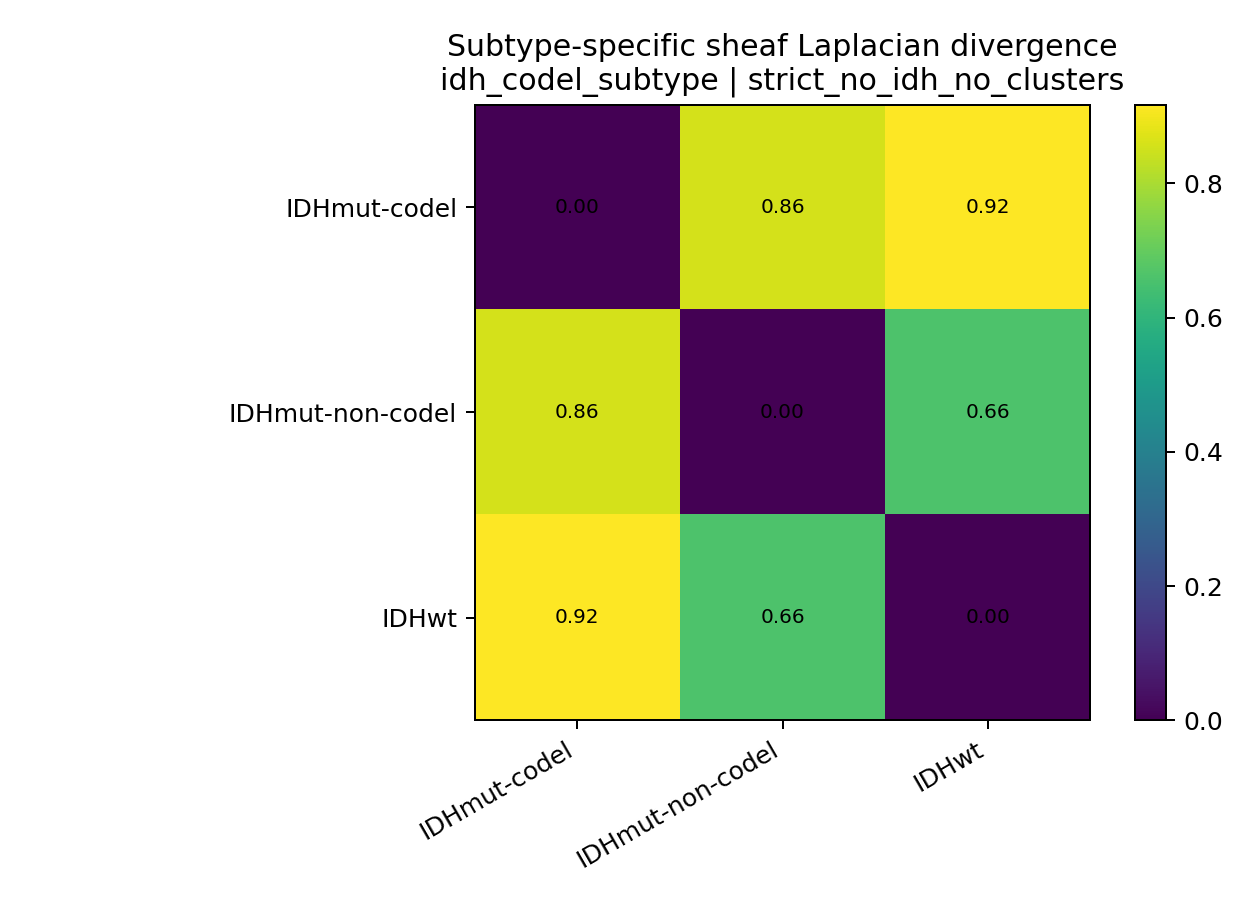
\includegraphics[width=0.92\linewidth]{../figures/phase4_divergence_heatmap_idh_codel_subtype_strict_no_idh_no_clusters.png}
\caption{Strict subtype-specific sheaf Laplacian divergence.}
\end{figure}

\begin{figure}[h!]
\centering
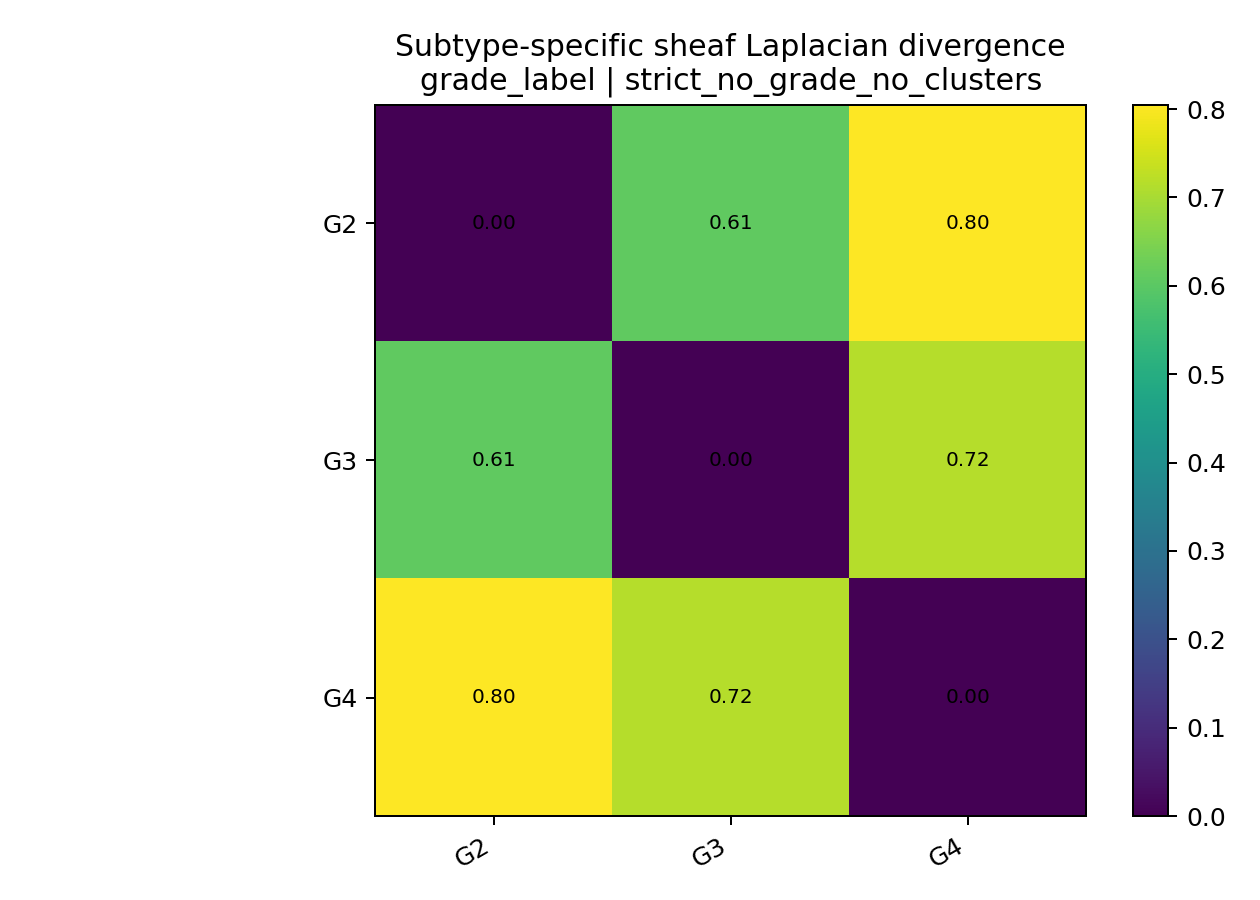
\includegraphics[width=0.92\linewidth]{../figures/phase4_divergence_heatmap_grade_label_strict_no_grade_no_clusters.png}
\caption{Strict grade-specific sheaf Laplacian divergence.}
\end{figure}

\begin{figure}[h!]
\centering
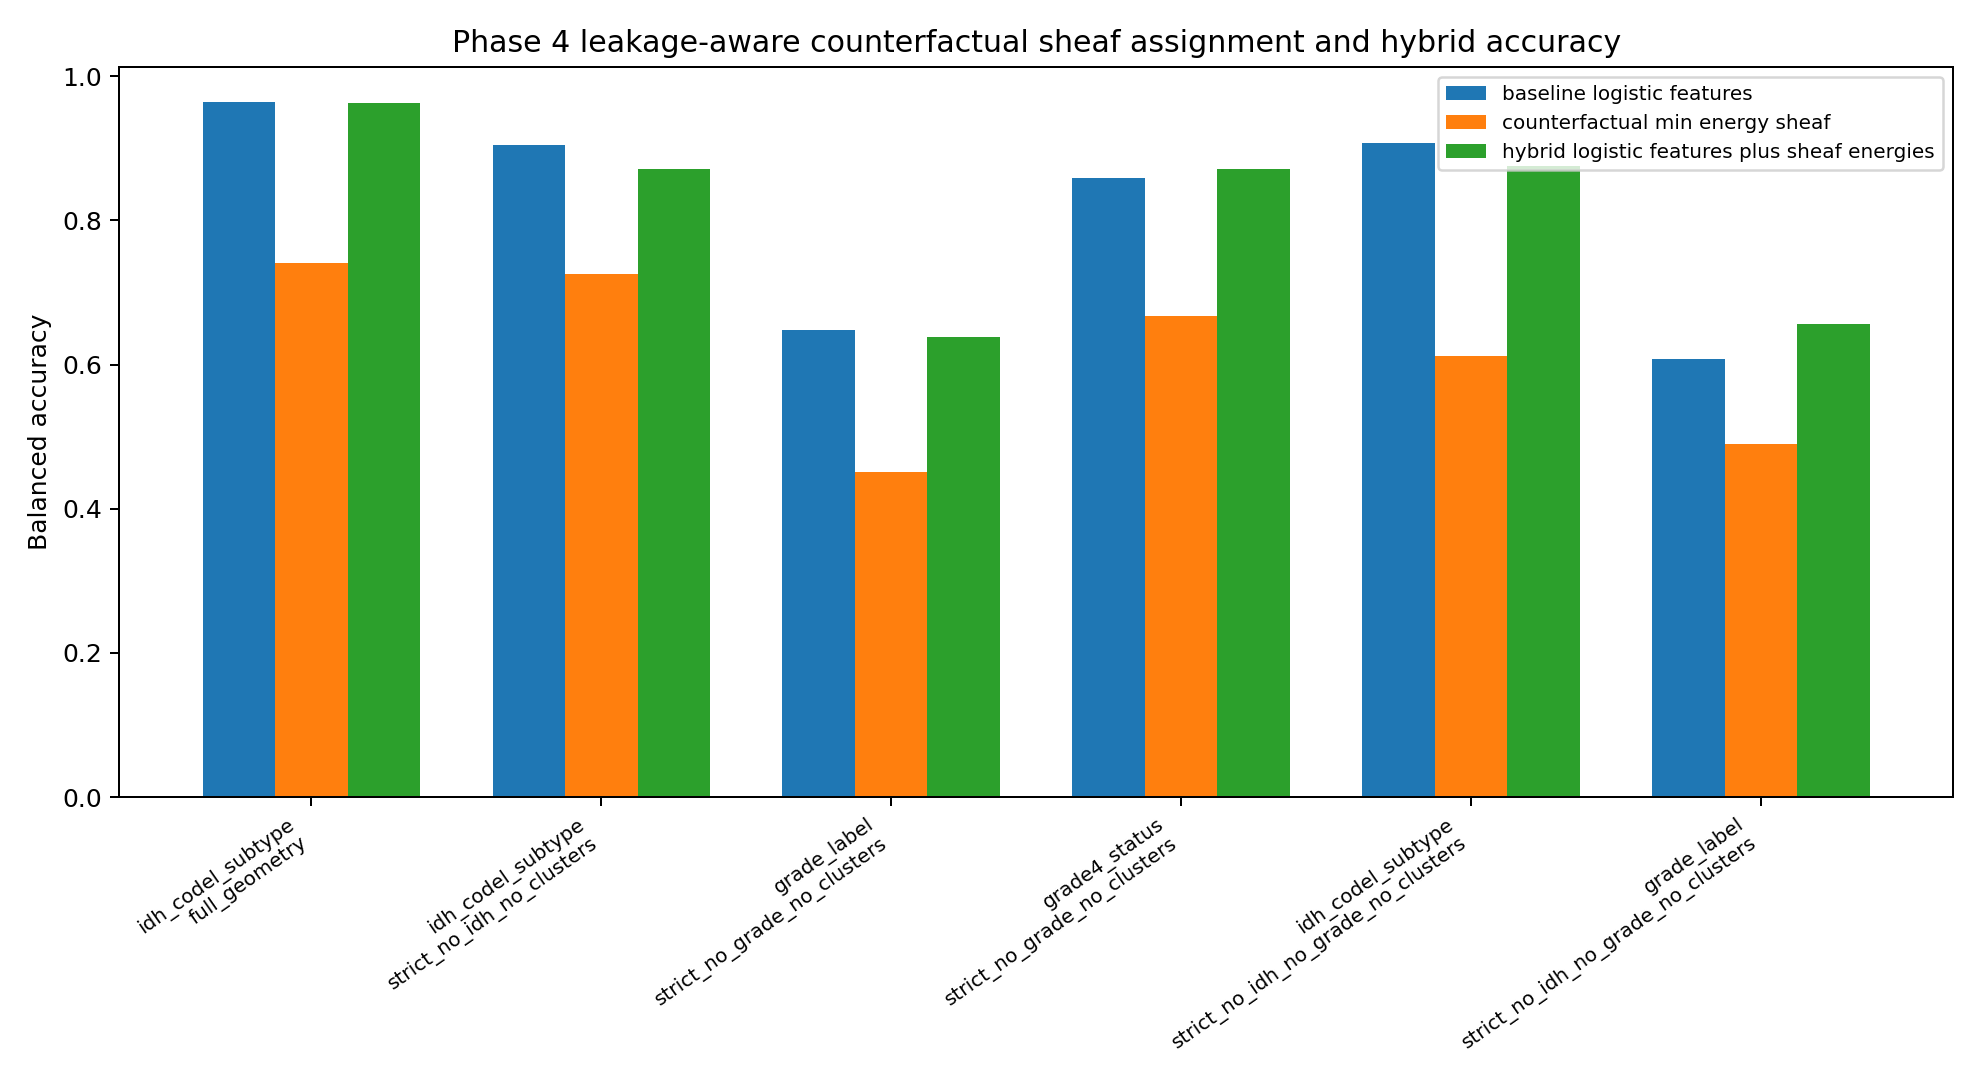
\includegraphics[width=0.98\linewidth]{../figures/phase4_balanced_accuracy_comparison.png}
\caption{Cross-validated balanced accuracy for baseline, counterfactual sheaf assignment, and hybrid sheaf-energy models.}
\end{figure}

\section{Interpretation}
Phase 4 creates a new object: a biological class is represented not only by feature means or classifier coefficients, but by a sheaf Laplacian $L_g$ encoding its learned consistency law. Patients are evaluated by their counterfactual energy under each law. This moves the project from feature integration toward geometric comparison of regulatory regimes.

\section{Limitations}
The current Phase 4 results are internal. They strengthen the method and generate new features, but external CGGA-style validation is still needed before making definitive state-of-the-art performance claims. The strongest current claim is methodological: subtype-specific sheaf Laplacians and counterfactual sheaf energies provide an interpretable alternative to ordinary graph aggregation.

\section{Next Required Work}
\begin{enumerate}[leftmargin=1.5em]
\item Add an external cohort and compute $E_g(p)$ under TCGA-trained sheaves.
\item Test whether subgroup Laplacian divergences replicate across cohorts.
\item Add pathway-level or gene-level nodes to move beyond the current three-node macro-sheaf.
\item Use permutation and bootstrap confidence intervals for every reported gain.
\end{enumerate}

\end{document}
